
%<<setup-child, include = FALSE>>=
%library(knitr)
%library(ggplot2)
%set_parent("../style/preamble.Rnw")
%options(digits = 16)
%@

\input{../../2021/style/preamble4tex}
% dependencies: amsmath, amssymb, dsfont
% math spaces
\ifdefined\N
\renewcommand{\N}{\mathds{N}} % N, naturals
\else \newcommand{\N}{\mathds{N}} \fi
\newcommand{\Z}{\mathds{Z}} % Z, integers
\newcommand{\Q}{\mathds{Q}} % Q, rationals
\newcommand{\R}{\mathds{R}} % R, reals
\ifdefined\C
\renewcommand{\C}{\mathds{C}} % C, complex
\else \newcommand{\C}{\mathds{C}} \fi
\newcommand{\continuous}{\mathcal{C}} % C, space of continuous functions
\newcommand{\M}{\mathcal{M}} % machine numbers
\newcommand{\epsm}{\epsilon_m} % maximum error

% counting / finite sets
\newcommand{\setzo}{\{0, 1\}} % set 0, 1
\newcommand{\setmp}{\{-1, +1\}} % set -1, 1
\newcommand{\unitint}{[0, 1]} % unit interval

% basic math stuff
\newcommand{\xt}{\tilde x} % x tilde
\newcommand{\argmin}{\mathop{\mathrm{arg\,min}}} % argmin
\newcommand{\argmax}{\mathop{\mathrm{arg\,max}}} % argmax
\newcommand{\argminlim}{\argmin\limits} % argmin with limits
\newcommand{\argmaxlim}{\argmax\limits} % argmax with limits
\newcommand{\sign}{\operatorname{sign}} % sign, signum
\newcommand{\I}{\mathbb{I}} % I, indicator
\newcommand{\order}{\mathcal{O}} % O, order
\newcommand{\bigO}{\mathcal{O}} % Big-O Landau
\newcommand{\littleo}{{o}} % Little-o Landau
\newcommand{\pd}[2]{\frac{\partial{#1}}{\partial #2}} % partial derivative
\newcommand{\floorlr}[1]{\left\lfloor #1 \right\rfloor} % floor
\newcommand{\ceillr}[1]{\left\lceil #1 \right\rceil} % ceiling
\newcommand{\indep}{\perp \!\!\! \perp} % independence symbol

% sums and products
\newcommand{\sumin}{\sum\limits_{i=1}^n} % summation from i=1 to n
\newcommand{\sumim}{\sum\limits_{i=1}^m} % summation from i=1 to m
\newcommand{\sumjn}{\sum\limits_{j=1}^n} % summation from j=1 to p
\newcommand{\sumjp}{\sum\limits_{j=1}^p} % summation from j=1 to p
\newcommand{\sumik}{\sum\limits_{i=1}^k} % summation from i=1 to k
\newcommand{\sumkg}{\sum\limits_{k=1}^g} % summation from k=1 to g
\newcommand{\sumjg}{\sum\limits_{j=1}^g} % summation from j=1 to g
\newcommand{\summM}{\sum\limits_{m=1}^M} % summation from m=1 to M
\newcommand{\meanin}{\frac{1}{n} \sum\limits_{i=1}^n} % mean from i=1 to n
\newcommand{\meanim}{\frac{1}{m} \sum\limits_{i=1}^m} % mean from i=1 to n
\newcommand{\meankg}{\frac{1}{g} \sum\limits_{k=1}^g} % mean from k=1 to g
\newcommand{\meanmM}{\frac{1}{M} \sum\limits_{m=1}^M} % mean from m=1 to M
\newcommand{\prodin}{\prod\limits_{i=1}^n} % product from i=1 to n
\newcommand{\prodkg}{\prod\limits_{k=1}^g} % product from k=1 to g
\newcommand{\prodjp}{\prod\limits_{j=1}^p} % product from j=1 to p

% linear algebra
\newcommand{\one}{\bm{1}} % 1, unitvector
\newcommand{\zero}{\mathbf{0}} % 0-vector
\newcommand{\id}{\bm{I}} % I, identity
\newcommand{\diag}{\operatorname{diag}} % diag, diagonal
\newcommand{\trace}{\operatorname{tr}} % tr, trace
\newcommand{\spn}{\operatorname{span}} % span
\newcommand{\scp}[2]{\left\langle #1, #2 \right\rangle} % <.,.>, scalarproduct
\newcommand{\mat}[1]{\begin{pmatrix} #1 \end{pmatrix}} % short pmatrix command
\newcommand{\Amat}{\mathbf{A}} % matrix A
\newcommand{\Deltab}{\mathbf{\Delta}} % error term for vectors

% basic probability + stats
\renewcommand{\P}{\mathds{P}} % P, probability
\newcommand{\E}{\mathds{E}} % E, expectation
\newcommand{\var}{\mathsf{Var}} % Var, variance
\newcommand{\cov}{\mathsf{Cov}} % Cov, covariance
\newcommand{\corr}{\mathsf{Corr}} % Corr, correlation
\newcommand{\normal}{\mathcal{N}} % N of the normal distribution
\newcommand{\iid}{\overset{i.i.d}{\sim}} % dist with i.i.d superscript
\newcommand{\distas}[1]{\overset{#1}{\sim}} % ... is distributed as ...


\begin{document}

\lecturechapter{5}{Introduction to Quadrature}
\lecture{CIM1 Statistical Computing}

% \begin{vbframe}{Notation}
% 
% \begin{itemize}
% \item $F(x)=\int f(x)dx$: Indefinite integral of $f(x)$
% \item $\kappa$: Condition number
% \item $\|f\|$: General norm of a function \\
% In this chapter: $\|f\|$ corresponds to the uniform norm $\|f\|_\infty = \max_x |f(x)|$
% \item $f \in \continuous^k$: $f$ is $k$ times continuously differentiable
% \item $\phi_{\mu, \sigma^2}, \Phi_{\mu, \sigma^2}$: Density/distribution function of a normally distributed random variable with expectation $\mu$ and variance $\sigma^2$
% \item $x \sim U(a, b)$: The random variable $x$ is uniformly distributed in the interval $[a, b]$
% \end{itemize}
% 
% \end{vbframe}

\begin{vbframe}{Motivation: Integrals in Statistics}

\begin{itemize}
\item Expectation of a random variable x with density $p$ that is transformed by a function $g$:
$$
\E_p[g(x)] = \int g(x)\cdot p(x)~dx
$$
\item Normalization constant in Bayes' theorem:
$$
\overset{Posterior}{p(\theta | x)} = \frac{\overset{Likelihood}{p(x | \theta)} \cdot \overset{Prior}{\pi(\theta)}}{\int p(x | \theta) \cdot \pi(\theta) ~ d\theta}
$$
\end{itemize}

The values of the integrals are often not elementary computable and must be calculated numerically on the computer.

\end{vbframe}

\begin{vbframe}{Integration}
\textbf{Goal:} Calculation of
$$
I(f) := \int_a^b f(x)dx
$$

\lz

We constrain ourselves to the concept of the \textbf{Riemann Integral}, which is defined by \textbf{Riemann sums}:

\begin{eqnarray*}
S(f) :&=& \sum_{k=0}^{n-1}(x_{k+1} - x_k) f(\xi_i)
\end{eqnarray*}

where $(x_0 = a, x_1, x_2, ..., x_{n-1}, x_n = b)$ is a partition of the interval $[a, b]$ and $\xi_i \in [x_i, x_{i+1}]$.

\framebreak

\begin{center}
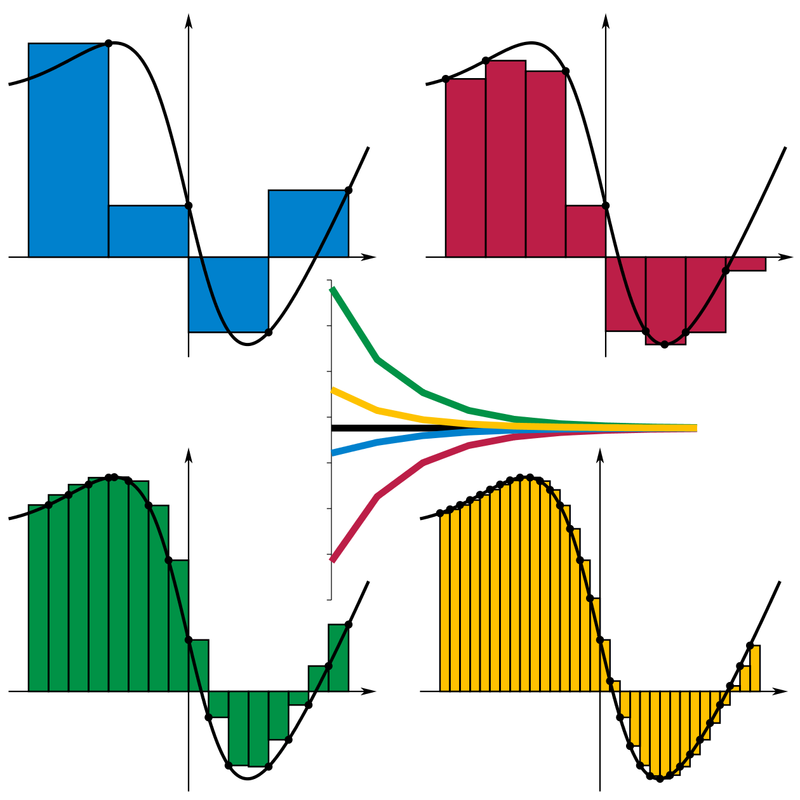
\includegraphics[width = 0.5\textwidth]{figure_man/riemannsums.png} \\
\begin{footnotesize}
\url{https://en.wikipedia.org/wiki/Riemann_sum}\\
Different methods for calculating Riemann sums.\\
Right (TL), left (BR), minimum (TR) and maximum (BL) method.

\end{footnotesize}
\end{center}

\framebreak

A function is Riemann-integrable on $[a, b]$, if the Riemann sums approach a fixed number (the value of the integral) as the partitions get finer, so the Riemann integral is the limit of the Riemann sums of a function for any arbitrary partition.

\lz

The operator $I(f)$, which assigns the value of the integral to an integrable function, is

\begin{itemize}
\item Linear, i.e. $I(\lambda f + \mu g) = \lambda I(f) + \mu I(g)$
\item Positive, i.e. $I(f) \ge 0$ for $f(x) \ge 0$ for all $x \in [a, b]$
\end{itemize}

\framebreak

% Das Integral existiert, falls die zugehörige Riemann-Summe für feinere Zerlegungen des Intervalls konvergieren, und ist dann definiert durch
%
% \begin{eqnarray*}
% I(f) = \int_a^b f(x)dx &:=& \lim_{n \to \infty} \sum_{k=0}^{n-1}(x_{k+1} - x_k) f(\xi_i).
% \end{eqnarray*}

The fundamental theorem of calculus states that the integral (in case of its existence) can be calculated using the indefinite integral

$$
I(f) = F(b) - F(a)
$$

However, for many interesting functions $f$ there is no elementarily representable integral $F$ and the direct analytical way is not possible.

\lz

\vspace*{-0.4cm}
\textbf{Examples}:
\begin{itemize}
\item $f(x)=e^{-\frac{x^2}2}$
\item Posterior calculations in Bayesian Statistics
\end{itemize}
\end{vbframe}


%\section{Numerisches Problem}

\begin{vbframe}{Numerical Problem}

%\vspace*{-0.3cm}
\textbf{Given:}
\begin{itemize}
\item Function $f$, can be evaluated anywhere (try to keep the number of evaluations small)
\item Interval of integration $[a, b]$
\item Error bound $\epsilon > 0$
\end{itemize}

\lz

\textbf{Searched:} $Q(f)$ with $\vert Q(f) - I(f) \vert \le \epsilon \cdot \vert I(f) \vert$

\lz

$E(f) := |Q(f) - I(f)|$ is referred to as $\textbf{Quadrature error}$.

% \lz
%
% Betrachten nur lineare Funktionale $Q$:
% $$
% Q(f) = \sum_{i=1}^n \omega_i f(x_i),
% $$
% mit Konstanten $\omega_i$, da Integration auch ein lineares Funktional ist.
\end{vbframe}

\begin{vbframe}{Condition of Integration}

\textbf{Question:} How much does the value of the integral change if we integrate a slightly transformed function $f + \Delta f$ instead of $f$?

\vspace*{-0.2cm}
\begin{center}
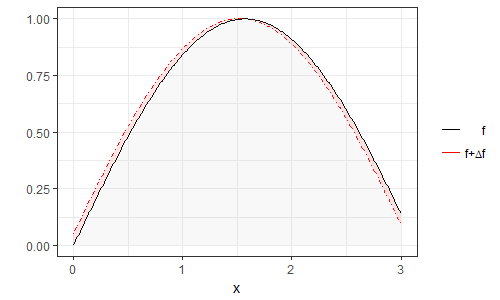
\includegraphics[width = .8\textwidth]{figure_man/konditionquadratur.png}
\end{center}

\framebreak

The relative condition is defined by the condition number $\kappa$, i.e. the smallest $\kappa \ge 0$, so that

$$
\frac{|I(f) - I(f + \Delta f)|}{|I(f)|} \le \kappa \frac{\|\Delta f\|_\infty}{\|f\|_\infty}
$$

It holds:

\vspace*{-0.5cm}
{\footnotesize
\begin{eqnarray*}
|I(f) - I(f + \Delta f)| &\overset{\text{linearity}}{=}& |I(f) - I(f) - I(\Delta f)| \\
  &=& \left| \int_a^b \Delta f(x)dx \right| \leq \int_a^b |\Delta f(x)|dx \\
  &\leq& (b - a) \underset{x \in [a, b]}{max}|\Delta f(x)| \\
  &=& (b - a) \| \Delta f \|_{\infty} \\[0.3cm]
\frac{|I(f) - I(f + \Delta f)|}{|I(f)|} &=& \frac{|I(\Delta f)|}{|I(f)|} \le (b - a) \frac{\|\Delta f\|_\infty}{|I(f)|} = (b - a) \frac{\|f\|_\infty}{|I(f)|} \frac{\|\Delta f\|_\infty}{\|f\|_\infty}
% |I(f) - I(f + \Delta f)|^2 &=& \left( \int_a^b \Delta f(x)dx \right)^2 \\
%   &\leq& \int_a^b (\Delta f(x))^2dx \cdot \int_a^b 1^2dx =
%   (b - a) \| f - (f + \Delta f) \|_2^2 \\[0.15cm]
% &\Rightarrow& |I(f) - I(f + \Delta f)| \leq
% \begin{cases}
% \sqrt{b - a}\cdot \| f - (f + \Delta f) \|_2 \\
% (b - a) \cdot \| f - (f + \Delta f) \|_{\infty}
% \end{cases}
\end{eqnarray*}
}

\framebreak

The condition number for the integration is therefore limited by

\vspace*{-0.2cm}
$$
\kappa = (b - a) \frac{\|f\|_\infty}{|I(f)|}
$$

In general, quadrature - in contrast to numerical differentiation - is well conditioned.
However, the upper bound for the condition is large if

\begin{itemize}
\item The function allows for large function values (large $\|f\|_\infty = \max_x f(x)$)
\item The absolute value of the integral is very small
\end{itemize}

If the problem is ill-conditioned, the result should be critically questioned (regardless of the stability of the algorithm).

\framebreak

\textbf{Example:}

Oscillating functions: $f_k(x) = \frac{(2k + 1)\pi}{2}\sin((2k+1)\pi x)$

\lz

The following holds: $I(f_k) = \int_0^1 f_k(x) dx = 1$ and $\|f_k\|_\infty = \frac{(2k+1)\pi}{2}$ and hence
\vspace{-0.1cm}
$$
\kappa = \frac{(2k+1)\pi}{2} \to \infty \quad \text{ for } k \to \infty
$$

\begin{center}
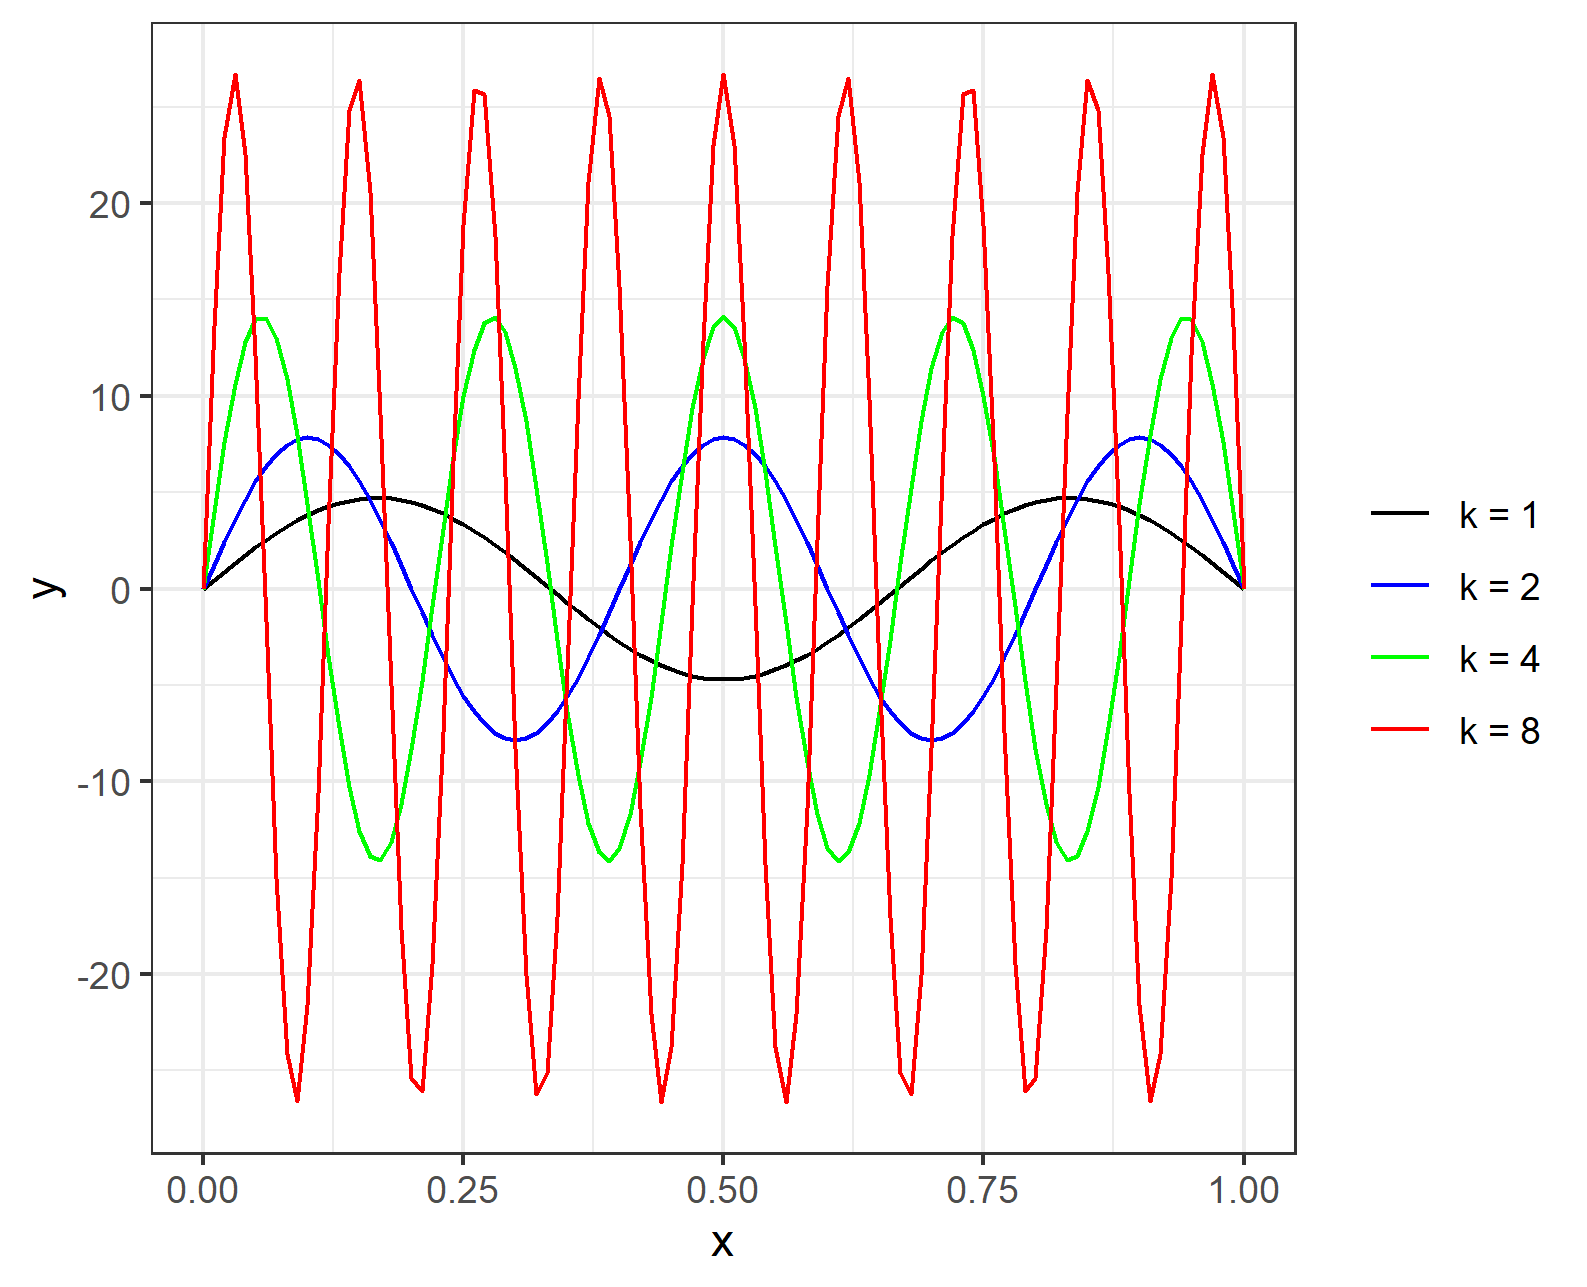
\includegraphics[width=0.45\textwidth]{figure_man/Example1.png}
\end{center}

%<<echo=F, out.width = '50%', fig.align = "center">>=
%f = function(x, k) {
%  (2 * k + 1) * base::pi / 2 * sin((2 * k + 1) * base::pi * x)
%}
%
%pl = ggplot(data.frame(x = c(0, 1)), aes(x = x)) + theme_bw()
%pl = pl + geom_path(aes(colour = "black"), stat = "function", fun = function(x) f(x, 1))
%pl = pl + geom_path(aes(colour = "blue"), stat = "function", fun = function(x) f(x, 2))
%pl = pl + geom_path(aes(colour = "green"), stat = "function", fun = function(x) f(x, 4))
%pl = pl + geom_path(aes(colour = "red"), stat = "function", fun = function(x) f(x, 8))
%pl = pl + scale_colour_identity(" ", guide = "legend",  labels = c("k = 1", "k = 2", "k = 4", "k = 8"),  breaks = c("black", "blue", "green", "red"))
%
%pl
%@


% \framebreak
%
%
% Ersetze $f$ durch Näherung, die leicht zu integrieren ist ({\em Polynome}).
%
% \lz
%
% Für lineare Funktionale $Q$ gilt:
%
% \begin{eqnarray*}
% | Q(f) - Q(g) | &=& | Q(f - g) | \\
% &\le& \sum_{i = 1}^n | \omega_i | | f(x_i) - g(x_i) | \\
% &\le& \left( \sum_{i = 1}^n | \omega_i | \right) \cdot \| f - \mathbf{g} \|_{\infty}
% \end{eqnarray*}
%
% \lz
%
% $Q$ liefert für konstante Funktionen, $f(x)\equiv \text{const}$, nur dann den richtigen Wert,
% falls $\sum_{i = 1}^n \omega_i = b - a$.
%
% \lz
%
% Es folgt: Kondition von $Q$ ist dann mit Kondition von $I$
% bzgl.\ der Sup-Norm identisch, wenn $\omega_i > 0 \,\, \forall i$.
% \end{vbframe}
%
% \begin{vbframe}{Konvergenzrate}
% \textbf{Annahme:} $\lim_{n \rightarrow \infty}Q_n(f) = I(f)$
%
% \begin{itemize}
%   \item \textbf{Lineare Konvergenz:} \\
%   Lineare Konvergenz liegt vor, falls es ein $0<c<1$ gibt, sodass
%   $$ \|Q_{n+1}(f) - I(f)\|\leq c\|Q_{n}(f) - I(f)\|. $$
%   \item \textbf{Konvergenz der Ordnung $p$:} \\
%   Eine Funktion konvergiert mit Ordnung $p \ (p>1)$, falls ein $c>0$
%   existiert, sodass
%   $$ \|Q_{n+1}(f) - I(f)\|\leq c\|Q_{n}(f) - I(f)\|^p. $$
%   Für $p=2$ spricht man dann beispielsweise von quadratischer Konvergenz.
% \end{itemize}

\end{vbframe}

% \begin{vbframe}{Beispielfunktion}
%
% Im folgenden werden verschiedene Methoden zur Integration vorgestellt und anhand der Funktion
%
% $$
% f(x) = - \sin(2(4x-2)) + 2 \exp(-16^2 (x - 0.5)^2) + 2.5
% $$
%
% illustriert.
%
%\section{Discretization}

\begin{vbframe}{Discretization}

\textbf{Discretization} is a central concept of numerical mathematics and the basis of many quadrature formulas. A continuous object (e.g. a function) is divided into $n$ \enquote{parts} to allow numerical evaluation and implementation.

\vspace*{0.2cm}

% The evaluation of a continuous function at only $n$ digits $\left((x_1, f(x_1)), ..., (x_n, f(x_n)\right)$ is a discretization.
%
% \vspace*{-0.1cm}

\begin{center}
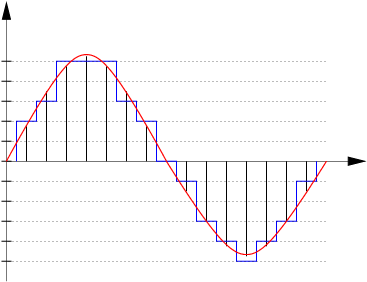
\includegraphics[width=0.4\textwidth]{figure_man/diskretisierung.png}\\
\begin{footnotesize}
Discretization of a continuous function.
\end{footnotesize}
\end{center}

\end{vbframe}

\begin{vbframe}{Error Analysis: Discretization Error}

Let $x_n$ be the numerical solution for the discretized object and $x^*$ the exact solution.

\lz

Due to the discretization an error is made, the so-called \textbf{truncation error}

$$
|x_n - x^*|
$$

Of course, this error should disappear for $n \to \infty$, the number of grid points in a discretization.

\lz

When using discretization, we are interested in how quickly the truncation error disappears.

\end{vbframe}

\begin{vbframe}{Convergence rates for discretization}

\textbf{Definition: }

The solution of the discretized problem $x_n$ converges with \textbf{order p} towards the solution of the continuous problem $x^*$ if there are constants $M > 0$ and $n_0 \in \N$, such that

$$
|x_n - x^*| \le M\cdot n^{-p} \quad \text{ for all } n > n_0
$$

or equivalently

$$
|x_n - x^*| \in \order{(n^{-p})}
$$

For $p = 1$ we speak of \textbf{linear} convergence, for $p = 2$ of \textbf{quadratic} convergence.

\end{vbframe}


% \begin{vbframe}{Numerical integration: two approaches}
% 
% We distinguish two approaches for the numerical calculation of the integral $\int_a^b f~dx$:
% 
% \begin{itemize}
% \item Identify an easily integrable function $\tilde f$ that is as similar as possible to $f$. The integral is then approximated by $Q(f) = I(\tilde f)$. \\[0.1cm]
% \textbf{Examples}: Newton-C\^{o}tes formulas, Laplace's method \\[0.4cm]
% \item Identify a sequence of estimates for the integral that converges for increasingly high resources (time, computing resources) towards the true value of the integral. \\[0.1cm]
% \textbf{Examples}: Monte Carlo integration
% \end{itemize}
% 
% \end{vbframe}



% \begin{vbframe}{Links- und Rechtssumme}
%
% Die erste und aufgrund der Definition des Riemann-Integrals naheliegende Methode ergibt sich über die Riemann-Summe, beispielsweise über \textbf{linke} und \textbf{rechte Riemann-Summen}
%
% $$
% R_n^l(f) = \sum\limits_{i = 0}^{n - 1} h f(a + ih), \quad R_n^r(f) =
%   \sum\limits_{i = 1}^{n} h f(a + ih),
% $$
% mit $h = (b - a) / n$.
%
% \lz
%
% Extrem einfach, aber konvergiert sehr langsam.
% % Extrem einfach, aber konvergiert, falls $f$ stetig, mit Konvergenzrate
% % $$
% % |I(f) - R_n(f)| \le (b - a) w(h), \,\, \mbox{ mit } \ w(h) = \sup\limits_{|x - y| < h}|f(x) - f(y)|.
% % $$
%
% \lz
%
% {\bf Bemerkung:} Wir betrachten vorerst nur gleich lange Intervalle (also $\omega_i = h$),
% Verallgemeinerung folgt.
%
% % \framebreak
%
%<<out.width = '90%', fig.align = "center", include = FALSE>>=
%fun = function(x) {
%  -1 * (sin(2 * (4*x - 2)) + 2 * exp(-16^2 * (x - 0.5)^2)) + 2.5
%}
%curve(fun, 0, 1, col = "red", ylab = "f(x)")
%@


%<<include = FALSE>>=
%riemann = function(f, a, b, n = 20, plot = FALSE, ...) {
%  h = (b - a) / n
%  x = a + 0:(n - 1) * h
%  R1 = sum(h * f(x))
%  R2 = sum(h * f(x + h))

%  if (plot) {
%    curve(f, a, b, ...)
%    rect(x, 0, x + h, f(x), col = rgb(.1, .1, .1, alpha = .3))
%    rect(x, 0, x + h, f(x + h), col = rgb(.1, .1, .1, alpha = .3))
%    curve(f, a, b, add = TRUE, col = "red", ...)
%  }
%  c(R1, R2)
%}
%@
%
% Ab hier kommt nicht immer R-Code für jede weitere Methode, siehe Übung / Tutorium!
%
% \end{vbframe}
%
% \begin{vbframe}{Links- und Rechtssumme Beispiel}
%
%<<fig.height=3, fig.width=5, include = FALSE>>=
%riemann(fun, 0, 1, n = 4, plot = TRUE)
%@

\framebreak

%<<include = F>>=
%riemann(fun, 0, 1, n = 10)
%riemann(fun, 0, 1, n = 100)
%riemann(fun, 0, 1, n = 1000)
%riemann(fun, 0, 1, n = 10000)
%@
% \end{vbframe}


% \end{vbframe}

\endlecture
\end{document}

